\documentclass[12pt]{scrartcl}

\usepackage[T1]{fontenc}
\usepackage[utf8]{inputenc}
\usepackage{amsmath}
\usepackage{amsfonts}
\usepackage{amssymb}
\usepackage{amsbsy}
\usepackage{graphicx}
\usepackage{float}
\usepackage{array}
\usepackage{booktabs}
\usepackage{multirow}
\usepackage{bm}
\usepackage{verbatim}
\usepackage[english]{babel}
\usepackage{color}
\usepackage{url}
\usepackage{fancybox}
\usepackage[stable]{footmisc}
\usepackage[format=plain,labelfont=bf]{caption}
\usepackage{fancyhdr}
\usepackage{natbib}
\usepackage{calc}
\usepackage{textcomp}
\usepackage[pdftex,pdfborder={0 0 0}]{hyperref}
\usepackage{pdfpages}
\usepackage{tikz}
\usetikzlibrary{shapes,backgrounds,fit,positioning,arrows,positioning,decorations.pathmorphing,decorations.pathreplacing,backgrounds}
\usepackage{accents}

\renewcommand*{\familydefault}{\sfdefault}

% Margins
\addtolength{\textheight}{1.0cm}
\addtolength{\oddsidemargin}{-0.5cm}
\addtolength{\evensidemargin}{-0.5cm}
\addtolength{\textwidth}{1.0cm}
\parindent=0em

% New math commands
\newcommand{\overbar}[1]{\mkern 1.5mu\overline{\mkern-1.5mu#1\mkern-1.5mu}\mkern 1.5mu}
\DeclareMathOperator{\diag}{diag}
\DeclareMathOperator{\Diag}{Diag}
\DeclareMathOperator{\tr}{tr}
\DeclareMathOperator{\var}{var}
\DeclareMathOperator{\Cov}{Cov}
\DeclareMathOperator{\Cor}{Cor}
\newcommand\independent{\protect\mathpalette{\protect\independenT}{\perp}}
\def\independenT#1#2{\mathrel{\setbox0\hbox{$#1#2$}%
\copy0\kern-\wd0\mkern4mu\box0}}

% Appropriate font for \mathcal{}
\DeclareSymbolFont{cmmathcal}{OMS}{cmsy}{m}{n}
\DeclareSymbolFontAlphabet{\mathcal}{cmmathcal}

% Set subscript and superscripts positions
\everymath{
\fontdimen13\textfont2=5pt
\fontdimen14\textfont2=5pt
\fontdimen15\textfont2=5pt
\fontdimen16\textfont2=5pt
\fontdimen17\textfont2=5pt
}

% Bibliography style
\setlength{\bibsep}{1pt}

% Part
\renewcommand\partheadstartvskip{\clearpage\null\vfil}
\renewcommand\partheadmidvskip{\par\nobreak\vskip 20pt\thispagestyle{empty}}
\renewcommand\partheadendvskip{\vfil\clearpage}
\renewcommand\raggedpart{\centering}

\begin{document}
\title{Filter banks localization}
\author{Benjamin Ménétrier}
\date{Last update: \today}

\thispagestyle{empty}

\maketitle
\begin{center}
Copyright \copyright 2025: Meteorologisk Institutt
\end{center}

%\tableofcontents

\section{Standard EnVar formulation}
For an ensemble $N$ backgrounds $\left\{\mathbf{x}^1,\dots,\mathbf{x}^N\right\}$, with $\mathbf{x}^k \in \mathbb{R}^n$, the standard EnVar formulation is given by:
\begin{align}
\label{eq:envar}
\mathbf{B} = \mathbf{X}\mathbf{X}^\mathrm{T} \circ \mathbf{L}
\end{align}
where:
\begin{itemize}
\item $\mathbf{B} \in \mathbb{R}^{n \times n}$ is the resulting background error covariance.
\item $\mathbf{X} \in \mathbb{R}^{n \times N}$ contains the normalized ensemble perturbations:
\begin{align}
X_{ij} = \frac{1}{\sqrt{N-1}} \left(x^j_i - \langle x_i \rangle\right)
\end{align}
with $\langle x_i \rangle$ denoting the ensemble mean:
\begin{align}
\langle x_i \rangle = \frac{1}{N} \sum_{j=1}^N x^j_i
\end{align}
\item $\mathbf{L} \in \mathbb{R}^{n \times n}$ is the localization matrix.
\item $\circ$ denotes a Schur product between matrices (element-by-element).
\end{itemize}
The square-root expression of \eqref{eq:envar}, transforming the control vector $\mathbf{v} \in \mathbb{R}^m$ into a control increment $\delta \mathbf{x} \in \mathbb{R}^n$, is given by:
\begin{align}
\delta \mathbf{x} = \sum_{j=1}^N \mathbf{X}_{:j} \circ \left(\mathbf{U} \mathbf{v}_j\right)
\end{align}
where:
\begin{itemize}
\item $\mathbf{X}_{:j} \in \mathbb{R}^n$ is the j$^\text{th}$ column of $\mathbf{X}$
\item $\mathbf{U} \in \mathbb{R}^{n \times m}$ is a square-root of the localization $\mathbf{L}$ such that $\mathbf{U} \mathbf{U}^\mathrm{T} = \mathbf{L}$.
\item $\mathbf{v}_j \in \mathbb{R}^{m/N}$ is the j$^\text{th}$ subvector of $\mathbf{v}$.
\end{itemize}

\section{Generalized EnVar formulation}
The standard EnVar formulation can be generalized by introducing two linear transforms $\mathbf{F} \in \mathbb{R}^{n \times \widehat{n}}$ and $\mathbf{F}^\dag \in \mathbb{R}^{\widehat{n} \times n}$:
\begin{align}
\widehat{\mathbf{B}} & = \mathbf{F} \left(\left(\mathbf{F}^\dag \mathbf{X}\right) \left(\mathbf{F}^\dag \mathbf{X}\right)^\mathrm{T} \circ \widehat{\mathbf{L}}\right) \mathbf{F}^\mathrm{T} \\
\delta \mathbf{x} & = \mathbf{F} \sum_{j=1}^N \left(\mathbf{F}^\dag \mathbf{X}_{:j}\right) \circ \left(\widehat{\mathbf{U}} \widehat{\mathbf{v}}_j\right)
\end{align}
where: 
\begin{itemize}
\item $\widehat{\mathbf{L}} \in \mathbb{R}^{\widehat{n} \times \widehat{n}}$ is the localization matrix in the transformed space.
\item $\widehat{\mathbf{U}} \in \mathbb{R}^{n \times \widehat{m}}$ is a square-root of the localization $\widehat{\mathbf{L}}$ such that $\widehat{\mathbf{U}} \widehat{\mathbf{U}}^\mathrm{T} = \widehat{\mathbf{L}}$.
\item $\widehat{\mathbf{v}}_j \in \mathbb{R}^{\widehat{m}/N}$ is the j$^\text{th}$ subvector of $\widehat{\mathbf{v}} \in \mathbb{R}^{\widehat{m}}$.
\end{itemize}
Let's analyse the asymptotic values if the ensemble size grows to infinity:
\begin{itemize}
\item The localization matrices $\mathbf{L}$ and $\widehat{\mathbf{L}}$ should converge to $\mathbf{1}_n$ and $\mathbf{1}_{\widehat{n}}$, respectively, where $\mathbf{1}_n \in \mathbb{R}^{n \times n}$ is a matrix filled with 1.
\item As a consequence:
\begin{align}
\lim_{N \rightarrow \infty} \mathbf{B} & = \mathbf{X} \mathbf{X}^\mathrm{T} \\
\lim_{N \rightarrow \infty} \widehat{\mathbf{B}} & = \left(\mathbf{F} \mathbf{F}^\dag \mathbf{X}\right) \left(\mathbf{F} \mathbf{F}^\dag \mathbf{X}\right)^\mathrm{T}
\end{align}
\item To ensure consistency, linear transforms $\mathbf{F}$ and $\mathbf{F}^\dag$ should not have an impact on the asymptotic background error covariance:
\begin{align}
\lim_{N \rightarrow \infty} \mathbf{B} = \lim_{N \rightarrow \infty} \widehat{\mathbf{B}}
\end{align}
so
\begin{align}
\mathbf{F} \mathbf{F}^\dag \mathbf{X} = \mathbf{X}
\end{align}
Thus, $\mathbf{F}^\dag$ should be a right-inverse of $\mathbf{F}$ in the ensemble perturbations space.
\end{itemize}

The content of $\mathbf{F}$ and $\mathbf{F}^\dag$ can be very diverse:
\begin{itemize}
\item A change of variables: for instance towards a better-suited humidity variable.
\item A inverse balance operator as in \citet{clayton_2012}, where the localization is applied on unbalanced variables and the balance operator is finally applied to get the increment.
\item A change of resolution as in \citet{kleist_2014a}, where the ensemble resolution is lower than the final increment one. In this case, $\mathbf{F}$ is an interpolation from low to high resolution, and the low-resolution perturbations $\mathbf{X}_\mathrm{LR}$ can be thought as the application of a coarsening operator $\mathbf{F}^\dag$ on virtual high-resolution perturbations $\mathbf{X}_\mathrm{HR}$ representing the same field:
\begin{align}
\mathbf{F} \mathbf{X}_\mathrm{LR} = \mathbf{F} \mathbf{F}^\dag \mathbf{X}_\mathrm{HR} = \mathbf{X}_\mathrm{HR}
\end{align}
\end{itemize}

\section{Filter banks localization}
In the filter banks localization (FBL) framework, we define three series of linear transforms:
\begin{itemize}
\item The low-pass filters $\left\{\mathbf{G}_1,\dots,\mathbf{G}_{P-1}\right\}$, where $\mathbf{G}_p \in \mathbb{R}^{\widehat{n}_p \times n}$.
\item The band-pass filters $\left\{\mathbf{H}_1,\dots,\mathbf{H}_P\right\}$, where $\mathbf{H}_p \in \mathbb{R}^{\widehat{n}_p \times n}$.
\item The interpolators $\left\{\mathbf{S}_1,\dots,\mathbf{S}_{P-1}\right\}$, where $\mathbf{S}_p \in \mathbb{R}^{n \times \widehat{n}_p}$.
\end{itemize}
where $\widehat{n}_p$ is the filtered space size at iteration $p$, with $\widehat{n}_P = n$.

\subsection{From explicit low-pass filters}
If the low-pass filters $\mathbf{G}_p$ are explicitly provided, the components of $\mathbf{F}^\dag$ are built recursively:
\begin{itemize}
\item The initial residual is given by the input state: $\overline{\mathbf{x}}_0 = \mathbf{x}$
\item At each iteration $1 \le p \le P-1$:
\begin{itemize}
\item The low-pass filter $\mathbf{G}_p$ is applied to the previous residual $\overline{\mathbf{x}}_{p-1} \in \mathbb{R}^n$ to produce the new filtered component $\widehat{\mathbf{x}}_p \in \mathbb{R}^{\widehat{n}_p}$:
\begin{align}
\label{eq:lp1}
\widehat{\mathbf{x}}_p = \mathbf{G}_p \overline{\mathbf{x}}_{p-1}
\end{align}
\item The new residual is computed from $\widehat{\mathbf{x}}_p$, interpolated at full resolution with $\mathbf{S}_p$:
\begin{align}
\label{eq:lp2}
\overline{\mathbf{x}}_p & = \overline{\mathbf{x}}_{p-1} - \mathbf{S}_p \widehat{\mathbf{x}}_p \\
& = \left(\mathbf{I}_n - \mathbf{S}_p \mathbf{G}_p\right) \overline{\mathbf{x}}_{p-1}
\end{align}
\end{itemize}
\end{itemize}
This construction can be illustrated as follows:
\begin{center}
\begin{tikzpicture}[scale=0.8,transform shape,auto,>=latex',line width=1pt]
\tikzstyle{block} = [draw, shape=rectangle, minimum height=0.8cm, minimum width=3.0cm]
\tikzstyle{branch}=[fill,shape=circle,minimum size=5pt,inner sep=0pt]

% Input
\node at (-2.5,0) (input) {$\mathbf{x}$};

% Filter 1
\node [block, right of=input, node distance=3.0cm] (F1) {$\mathbf{G}_1$};
\node [right of=F1, node distance=2.7cm, yshift=-0.02cm] (F1x) {$\widehat{\mathbf{x}}_1$};
\node [block, below of=F1, node distance=1.0cm] (ImF1) {$\mathbf{I}_n - \mathbf{S}_1 \mathbf{G}_1$};
\node [right of=ImF1, node distance=2.7cm, yshift=-0.02cm] (ImF1x) {$\overline{\mathbf{x}}_1$};
\path (input) -- coordinate(branch1) (F1);
\draw[->] (input) -- (F1);
\draw[->] (F1) -- ([yshift=0.02cm]F1x.west);
\draw[->] (ImF1) -- ([yshift=0.02cm]ImF1x.west);
\draw[->] (branch1) node[branch] {} |- (ImF1);

% Filter 2
\node [block, right of=ImF1, node distance=5.8cm] (F2) {$\mathbf{G}_2$};
\node [right of=F2, node distance=2.7cm, yshift=-0.02cm] (F2x) {$\widehat{\mathbf{x}}_2$};
\node [block, below of=F2, node distance=1.0cm] (ImF2) {$\mathbf{I}_n - \mathbf{S}_2 \mathbf{G}_2$};
\node [right of=ImF2, node distance=2.7cm, yshift=-0.02cm] (ImF2x) {$\overline{\mathbf{x}}_2$};
\path (ImF1x) -- coordinate(branch2) (F2);
\draw[->] (ImF1x) -- (F2);
\draw[->] (F2) -- ([yshift=0.02cm]F2x.west);
\draw[->] (ImF2) -- ([yshift=0.02cm]ImF2x.west);
\draw[->] (branch2) node[branch] {} |- (ImF2);

% Etc
\node [right of=ImF2x, node distance=2.0cm] (dots1) {\dots};
\node [below of=dots1, node distance=1.0cm] (dots2) {\dots};
\path (ImF2x) -- coordinate(branch3) (dots1);
\draw[->] (ImF2x) -- (dots1);
\draw[->] (branch3) node[branch] {} |- (dots2);

\end{tikzpicture}
\end{center}

Integrating recursively, the residual at iteration $p$ becomes:
\begin{align}
\label{eq:lp3}
\overline{\mathbf{x}}_p & = \left(\mathbf{I}_n - \mathbf{S}_p \mathbf{G}_p\right) \left(\mathbf{I}_n - \mathbf{S}_{p-1} \mathbf{G}_{p-1}\right) \dots \left(\mathbf{I}_n - \mathbf{S}_1 \mathbf{G}_1\right) \mathbf{x} \nonumber \\
& = \displaystyle \prod_{q=1}^p \left(\mathbf{I}_n - \mathbf{S}_q \mathbf{G}_q\right) \mathbf{x}
\end{align}
and from \eqref{eq:lp1}, we obtain the filtered component at iteration $p$:
\begin{align}
\label{eq:lp4}
\widehat{\mathbf{x}}_p & = \mathbf{G}_p \prod_{q=1}^{p-1} \left(\mathbf{I}_n - \mathbf{S}_q \mathbf{G}_q\right) \mathbf{x}
\end{align}

By definition, the band-pass filter $\mathbf{H}_p$ applied directly to the input state $\mathbf{x}$ should provide the filtered component $\widehat{\mathbf{x}}_p$:
\begin{align}
\mathbf{H}_p \mathbf{x} = \widehat{\mathbf{x}}_p
\end{align}
Combining this equation with \eqref{eq:lp4}, we get an equivalence between low-pass and band-pass filters for $1 \le p \le P-1$:
\begin{align}
\mathbf{H}_p = \mathbf{G}_p \prod_{q=1}^{p-1} \left(\mathbf{I}_n - \mathbf{S}_q \mathbf{G}_q\right)
\end{align}
The last band-pass filter $\mathbf{H}_P$ applied to the input state should produce the last residual:
\begin{align}
\mathbf{H}_P \mathbf{x} & = \overline{\mathbf{x}}_{P-1}
\end{align}
So equation \eqref{eq:lp3} gives:
\begin{align}
\mathbf{H}_P = \prod_{q=1}^{P-1} \left(\mathbf{I}_n - \mathbf{S}_q \mathbf{G}_q\right)
\end{align}
But integrating equation \eqref{eq:lp2} recursively, the last residual can also be expressed as:
\begin{align}
\overline{\mathbf{x}}_{P-1} & = \mathbf{x} - \sum_{p=1}^{P-1} \mathbf{S}_p \widehat{\mathbf{x}}_p \nonumber \\
 & = \mathbf{x} - \sum_{p=1}^{P-1} \mathbf{S}_p \mathbf{H}_p \mathbf{x}
\end{align}
Which proves that the last band-pass filter is actually the complement of the sum of all the previous band-pass filters combined with the corresponding interpolations:
\begin{align}
\mathbf{H}_P = \mathbf{I}_n - \sum_{p=1}^{P-1} \mathbf{S}_p \mathbf{H}_p
\end{align}
Figure \ref{fig:lp_to_bp} shows an example of spectra for explicit low-pass filters with Gaussian shapes, resulting for instance from a diffusion process, and their equivalent band-pass filters.\\
\begin{center}
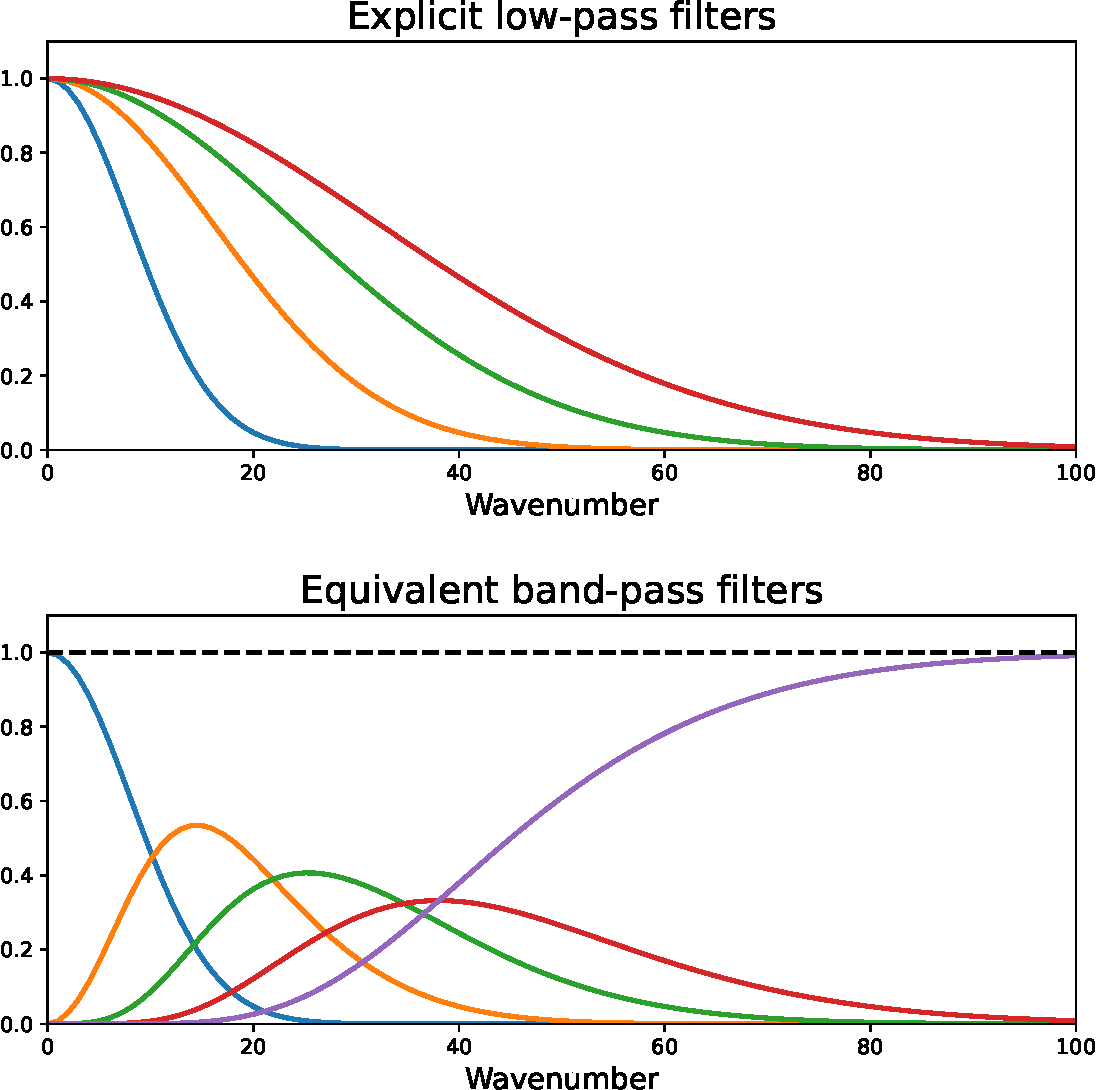
\includegraphics[width=0.49\linewidth]{lp_to_bp.pdf}
\captionof{figure}{Spectra of explicit low-pass filters (top) and their equivalent band-pass filters (bottom). The dashed black line shows the sum of all the band-pass filters. \label{fig:lp_to_bp}}
\end{center}

Formally, the linear transform $\mathbf{F}^\dag$ can be written as:
\begin{align}
\mathbf{F}^\dag = \left( \begin{array}{c}
\mathbf{H}_1 \\
\mathbf{H}_2 \\
\vdots \\
\mathbf{H}_P
\end{array}
\right)
\end{align}
where the total size of the transformed space is $\displaystyle \widehat{n} = \sum_{p=1}^P n_p$. The left-inverse of $\mathbf{F}^\dag$ is simply:
\begin{align}
\mathbf{F} = \left(\mathbf{S}_1 \mathbf{S}_2 \dots \mathbf{S}_{P-1} \mathbf{I}_n\right)
\end{align}

\subsection{From explicit band-pass filters}
Starting from explicit band-pass filters $\mathbf{H}_p$, it is easier to construct the linear transform $\mathbf{F}^\dag$. It is also possible to retrieve the corresponding low-pass filters iteratively:
\begin{itemize}
\item The initial low-pass filter is equal to the initial band-pass filter:
\begin{align}
\mathbf{G}_1 = \mathbf{H}_1
\end{align}
\item For $2 \le p \le P-1$, the low-pass filter $\mathbf{G}_p$ is given by:
\begin{align}
\mathbf{G}_p & = \mathbf{H}_p \left(\mathbf{I}_n - \mathbf{S}_1 \mathbf{G}_1\right)^\dag \left(\mathbf{I}_n - \mathbf{S}_2 \mathbf{G}_2\right)^\dag \dots \left(\mathbf{I}_n - \mathbf{S}_{p-1} \mathbf{G}_{p-1}\right)^\dag \nonumber \\
& = \mathbf{H}_p \prod_{q=1}^{p-1} \left(\mathbf{I}_n - \mathbf{S}_{p-q} \mathbf{G}_{p-q}\right)^\dag
\end{align}
\end{itemize}
where $\left(\mathbf{I}_n - \mathbf{S}_p \mathbf{G}_p\right)^\dag$ is a right-inverse of $\left(\mathbf{I}_n - \mathbf{S}_p \mathbf{G}_p\right)$. Figure \ref{fig:bp_to_lp} shows an example of spectra for explicit band-pass filters with wavelet-like shapes, and their equivalent low-pass filters.\\
\begin{center}
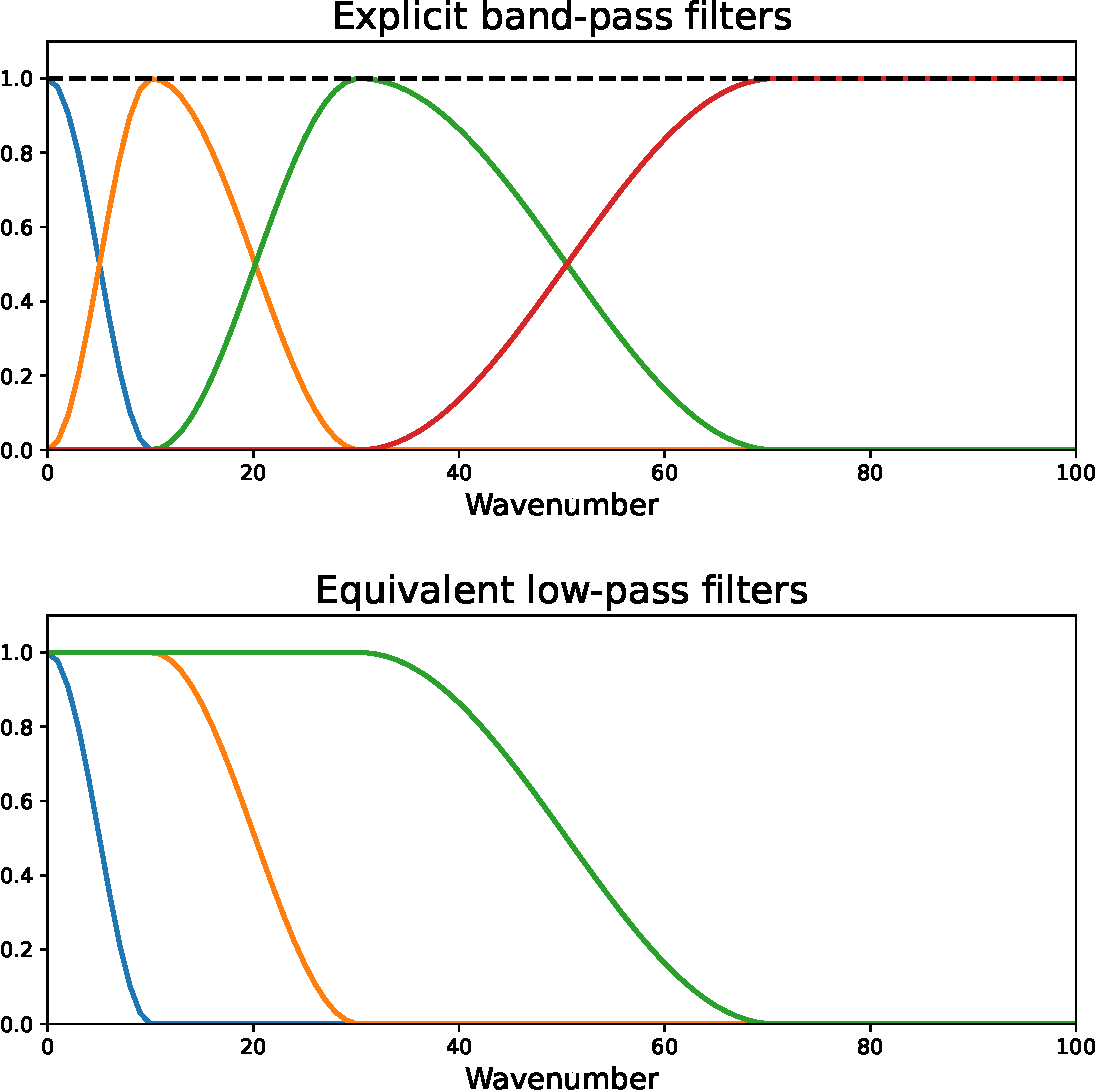
\includegraphics[width=0.49\linewidth]{bp_to_lp.pdf}
\captionof{figure}{Spectra of explicit band-pass filters (top) and their equivalent low-pass filters (bottom). The dashed black line shows the sum of all the band-pass filters. \label{fig:bp_to_lp}}
\end{center}


\subsection{Scale-dependent localization}
The standard scale-dependent localization (SDL) described in \citet{buehner_2015b} can be seen as a special case of filter banks localization (FBL), where:
\begin{itemize}
\item All the components have the same grid size $\widehat{n}_p = n$, so the size of the transformed space is $\widehat{n} = Pn$.
\item There is no interpolation: $\mathbf{S}_p = \mathbf{I}_n$
\end{itemize}
Many implementations are possible in this case:
\begin{itemize}
\item Explicit band-pass filters $\mathbf{H}_p$ in spectral space: $\mathbf{H}_p = \mathbf{T}^{-1} \mathbf{D}_p \mathbf{T}$ where $\mathbf{T}$ is a spectral transform and $\mathbf{D}_p$ is the diagonal analytical filter defining waveband $p$.
\item Explicit low-pass filters $\mathbf{G}_p$ based on a diffusion process using increasing diffusion length-scales.
\end{itemize}

\subsection{Interpolation-based filter banks localization}
The interpolation-based filter banks localization (IFBL) is a special case of the filter banks localization (FBL) where the low-pass filter $\mathbf{G}_p$ for component $p$ is given by:
\begin{align}
\mathbf{G}_p = \mathbf{N}_p \mathbf{S}_p^\mathrm{T}
\end{align}
where the i$^\text{th}$ coefficient of the diagonal normalization matrix $\mathbf{N}_p$ is equal to the inverse of the i$^\text{th}$ coefficient of the vector $\mathbf{S}_p^\mathrm{T} \mathbf{1}_n$.

\subsection{Methods comparison}
To illustrate the similarities and differences between the SDL and IFBL methods, we start from a random field $\mathbf{x}$ with different scales depending on the location in Figure \ref{fig:init}. In Figure \ref{fig:filt_1}, the filtered field $\widehat{\mathbf{x}}_1$ at low resolution captures the largest scales of the signal. These scales are removed in the corresponding residual $\overline{\mathbf{x}}_1$, in Figure \ref{fig:res_1}. In Figure \ref{fig:filt_2}, the filtered field $\widehat{\mathbf{x}}_2$ at intermediate resolution captures the intermediate scales of the signal. Only the smallest scale are left in the final residual $\overline{\mathbf{x}}_2$, in Figure \ref{fig:res_2}.\\
$  $\\
Here, the SDL uses the \texttt{scipy.ndimage.gaussian\_filter} function of \texttt{Python} for $\mathbf{G}_p$. The IFBL uses a standard bilinear interpolation. The filtering scales of the SDL and the low-resolution grids of the IFBL have been briefly tuned to yield visually similar results.

\begin{center}
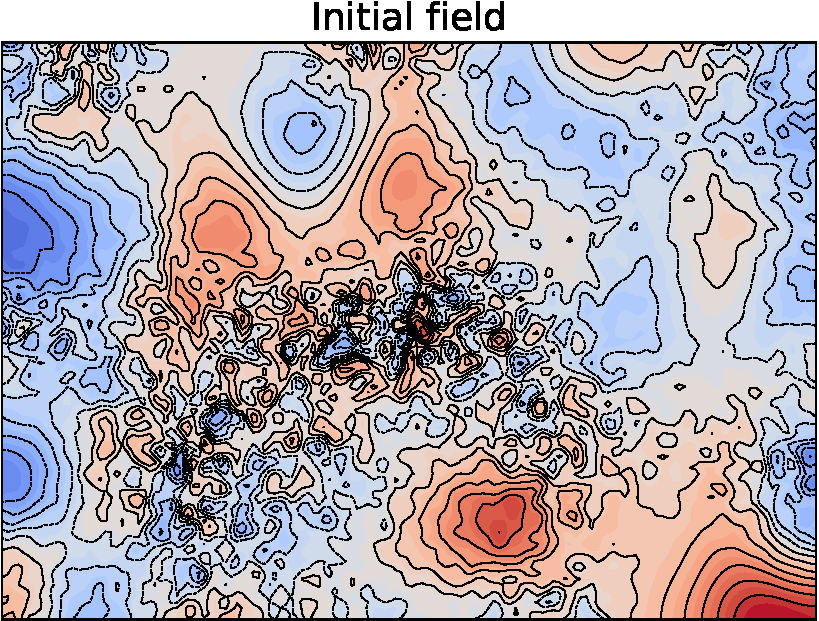
\includegraphics[width=0.49\linewidth]{init.pdf}
\captionof{figure}{Random field with different scales depending on the location. \label{fig:init}}
\end{center}

\begin{center}
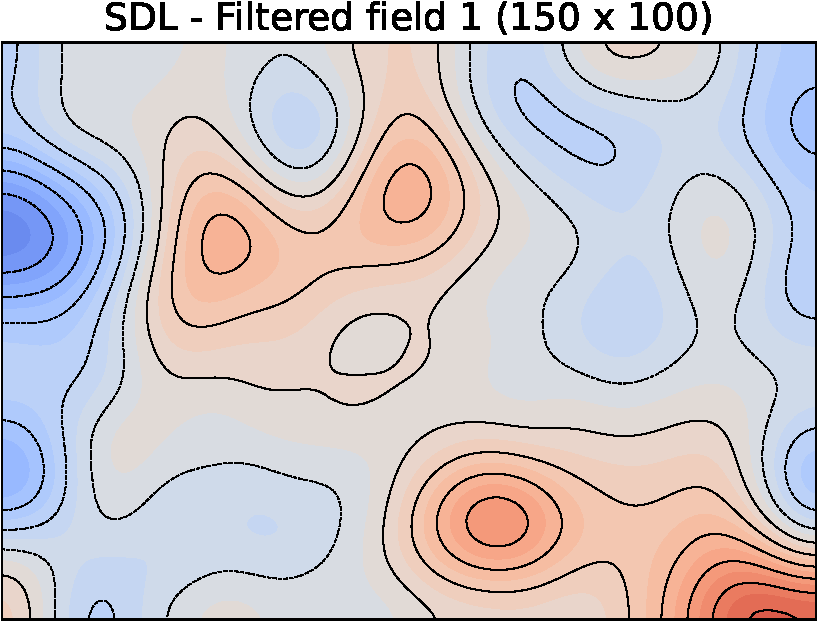
\includegraphics[width=0.49\linewidth]{sdl_1_filt.pdf}
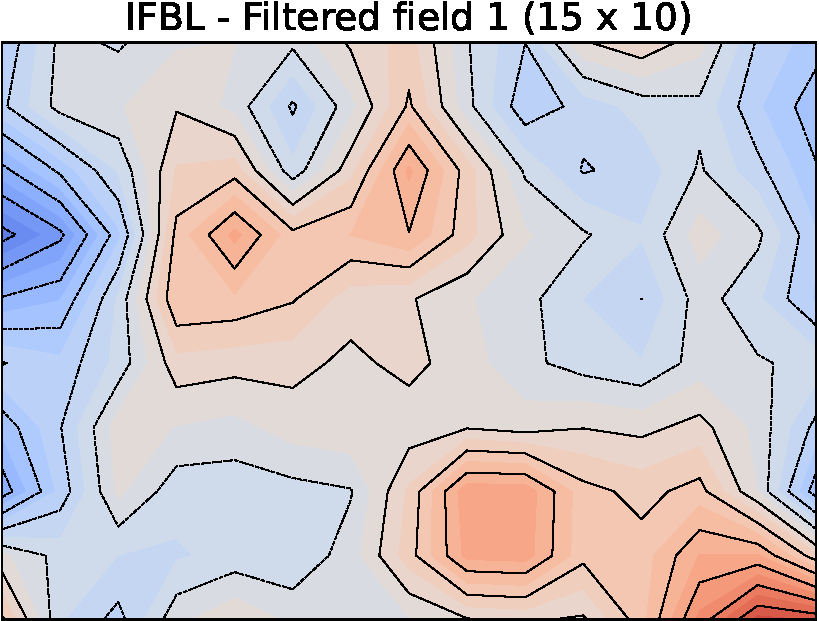
\includegraphics[width=0.49\linewidth]{ifbl_1_filt.pdf}
\captionof{figure}{Filtered field at low-resolution 1 with SDL (left) and IFBL (right)and corresponding residual (right). \label{fig:filt_1}}
\end{center}

\begin{center}
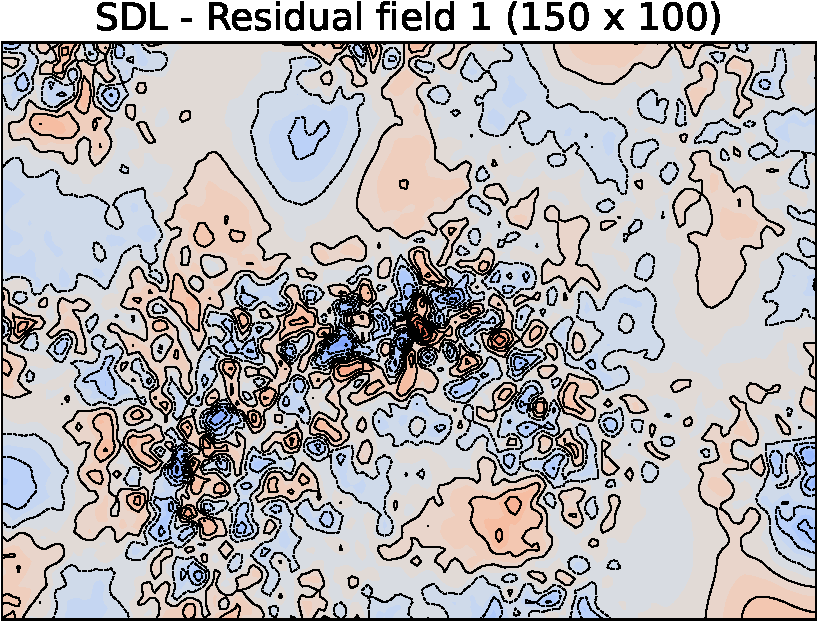
\includegraphics[width=0.49\linewidth]{sdl_1_res.pdf}
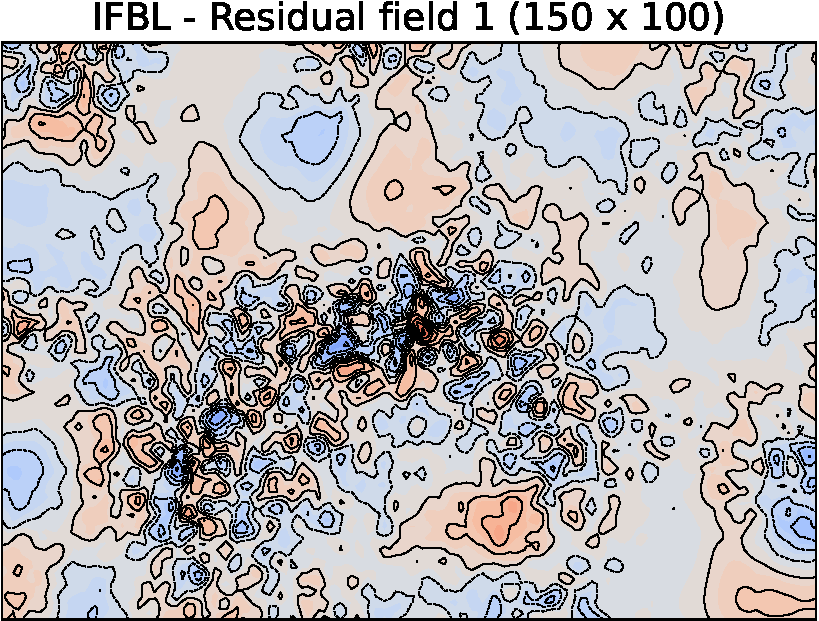
\includegraphics[width=0.49\linewidth]{ifbl_1_res.pdf}
\captionof{figure}{Residual field at low-resolution 1 with SDL (left) and IFBL (right). \label{fig:res_1}}
\end{center}

\begin{center}
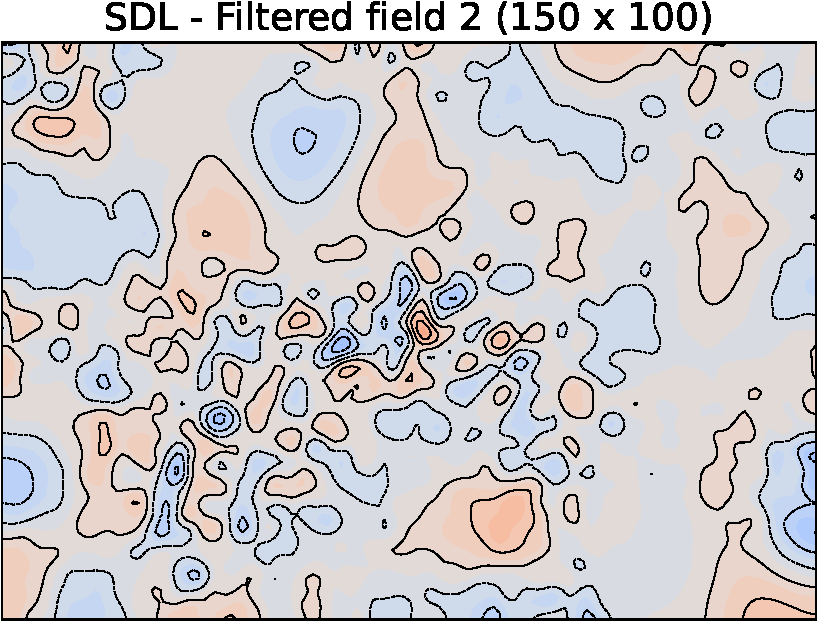
\includegraphics[width=0.49\linewidth]{sdl_2_filt.pdf}
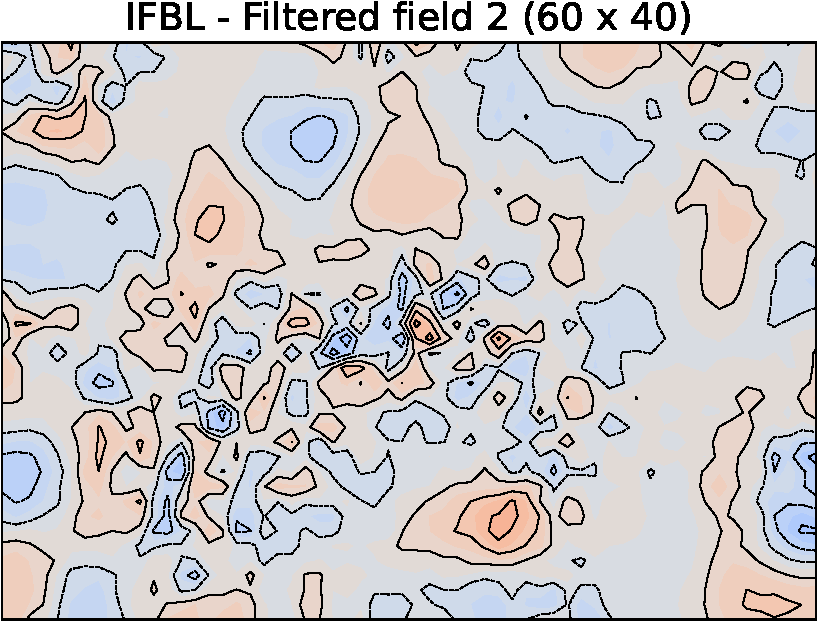
\includegraphics[width=0.49\linewidth]{ifbl_2_filt.pdf}
\captionof{figure}{Filtered field at low-resolution 2 with SDL (left) and IFBL (right)and corresponding residual (right). \label{fig:filt_2}}
\end{center}

\begin{center}
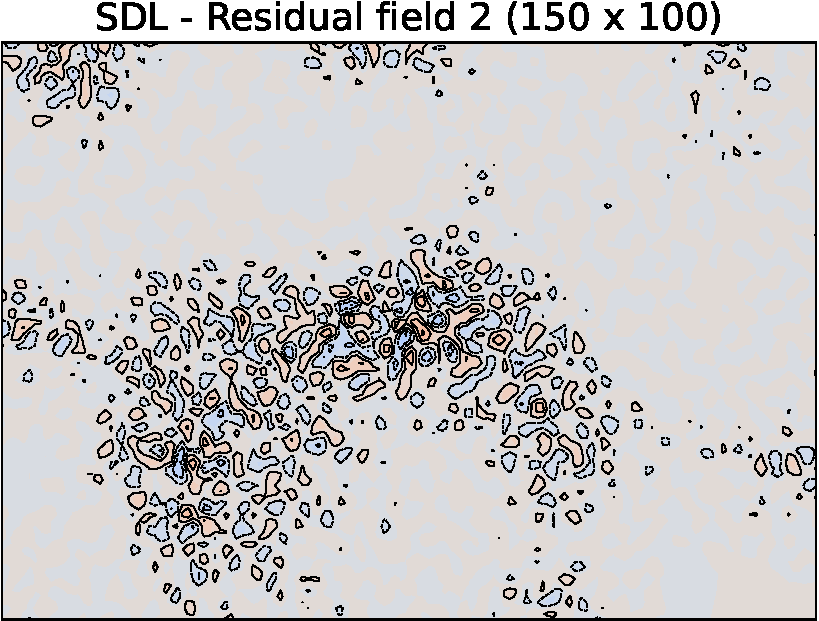
\includegraphics[width=0.49\linewidth]{sdl_2_res.pdf}
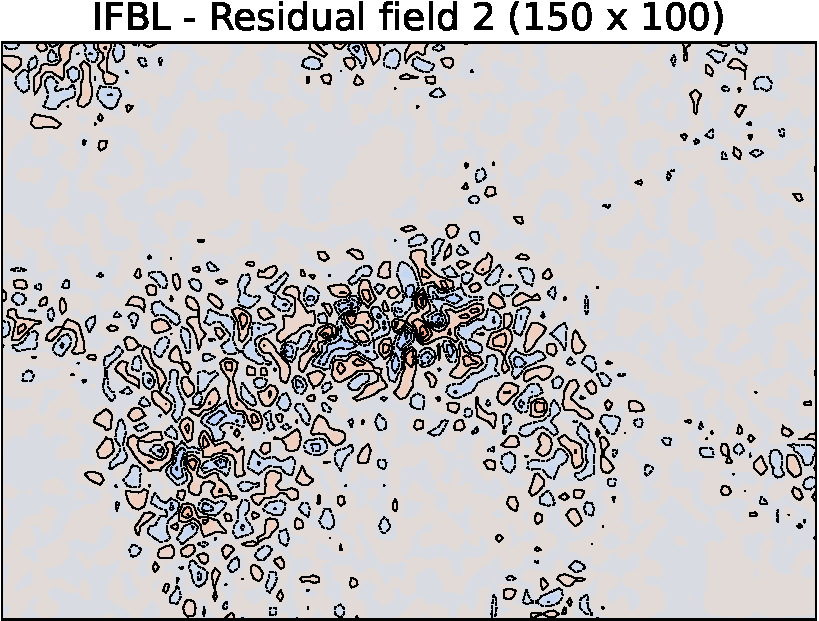
\includegraphics[width=0.49\linewidth]{ifbl_2_res.pdf}
\captionof{figure}{Residual field at low-resolution 2 with SDL (left) and IFBL (right). \label{fig:res_2}}
\end{center}

The interpolation-based filter banks localization (IFBL) leads to a smaller size of the transformed space $\widehat{n}$ than the scale-dependent localization (SDL), reducing the required memory for the same number of components. Also, the choice of the grids for the low-resolution components is completely flexible. Once the interpolation from low resolution to full resolution and its adjoint are available, the construction of the low-pass filter is straightforward. However, the IFBL requires that the localization matrix is applied in the geoemetry of each component, which is more complicated but also cheaper because the localization is applied at lower resolution.

% Bibliography
\bibliographystyle{mybib-en}
\bibliography{filter_banks_localization}
\end{document}
